\begin{pa} \label{PA:10.4}  Let $f(x,y) = 6 - \frac{x^2}2 - y^2$, and let $(x_0,y_0)
  = (1,1)$.
\ba
\item Evaluate $f(x,y) = 6 - \frac{x^2}2 - y^2$ and its partial derivatives at $(x_0,y_0)$;  that is, find $f(1,1)$, $f_x(1,1)$, and $f_y(1,1)$.

\item We know one point on the tangent plane;  namely, the $z$-value of the tangent
  plane agrees with the $z$-value on the graph of the function $f(x,y) = 6 - \frac{x^2}2 - y^2$ at the point $(x_0,
  y_0)$.  In other words, both the tangent plane and the graph of the function $f$ contain the point $(x_0, y_0, z_0)$. Use this observation to determine $z_0$ in the expression
  $z = z_0 + a(x-x_0) + b(y-y_0)$.

\item Sketch the traces of the function $f(x,y) = 6 - \frac{x^2}2 - y^2$ for $y=y_0=1$ and $x=x_0=1$
  below in Figure \ref{F:10.4.traces}.  

  \begin{figure}[ht]
    \begin{center}
      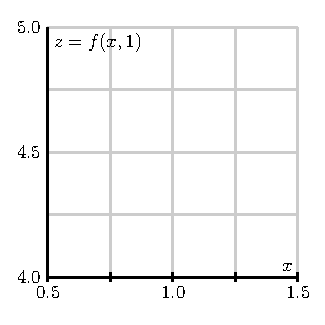
\includegraphics{figures/fig_10_4_tangent_trace_y.eps}
      \hspace*{20pt}
      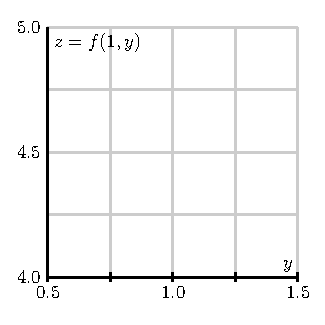
\includegraphics{figures/fig_10_4_tangent_trace_x.eps}
    \end{center}
    \caption{The traces of $f(x,y)$ with $y=y_0=1$ and $x=x_0=1$.}
    \label{F:10.4.traces}
  \end{figure}

\item Determine the equation of the tangent line of the trace that you sketched in the previous part with $y=1$ (in the $x$ direction) at the point $x_0=1$.  

  \begin{figure}[ht]
    \begin{center}
      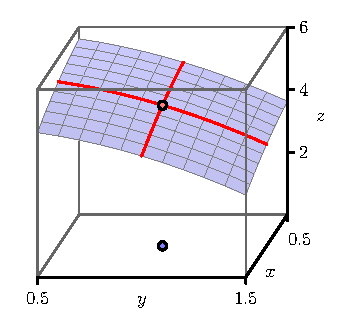
\includegraphics{figures/fig_10_4_tangent_5.eps}
      \hspace*{20pt}
      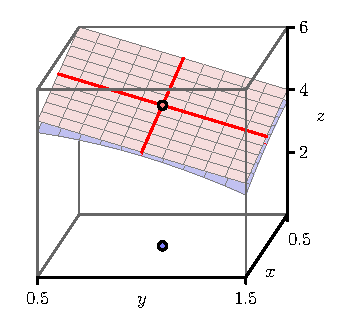
\includegraphics{figures/fig_10_4_tangent_6.eps}
    \end{center}
    \caption{The traces of $f(x,y)$ and the tangent plane.}
    \label{F:10.4.tangent.traces}
  \end{figure}
  
\item Figure \ref{F:10.4.tangent.traces} shows the traces of the
  function and the traces of the tangent plane.  Explain how the
  tangent line of the trace of $f$, whose equation you found in the
  last part of this 
  activity, is related to the tangent plane.  How does this
  observation help you determine the constant $a$ in the equation for the tangent plane $z
  = z_0+a(x-x_0) + b(y-y_0)$?  (Hint: How do you think $f_x(x_0,y_0)$ should be related to $z_x(x_0,y_0)$?)



\item In a similar way to what you did in (d), determine the equation of the tangent line of the
  trace with $x=1$ at the point $y_0=1$.  Explain how this tangent
  line is related to the tangent plane, and use this observation to
  determine the constant $b$ in the equation for the tangent plane
  $z=z_0+a(x-x_0) + b(y-y_0)$. (Hint: How do you think $f_y(x_0,y_0)$ should be related to $z_y(x_0,y_0)$?)

\item Finally, write the equation $z=z_0 + a(x-x_0) + b(y-y_0)$ of the tangent
  plane to the graph of $f(x,y)=6-x^2/2 - y^2$ at the point
  $(x_0,y_0)=(1,1)$. 

\ea

\end{pa}

\begin{activitySolution} 
\ba
\item Since $f_x(x,y) = -x$ and $f_y(x,y) = -2y$ we have $f(1,1) = \frac{9}{2}$, $f_x(1,1) = -1$, and $f_y(1,1) = -2$. 

\item Since $f(1,1) = \frac{9}{2}$ we must have $z_z=\frac{9}{2}$. 

\item 
%The traces in the $x$ and $y$ directions are shown below.  

%  \begin{figure}[ht]
%    \begin{center}
%      \resizebox{!}{2.5in}{\includegraphics{figures/fig_10_4_tangent_trace_x_sol.eps}}
%      \hspace*{20pt}
%      \resizebox{!}{2.5in}{\includegraphics{figures/fig_10_4_tangent_trace_y_sol.eps}}
 %   \end{center}
%    \caption{The traces of $f(x,y)$ with $y=y_0=1$ and $x=x_0=1$.}
%    \label{F:10.4.traces_sol}
%  \end{figure}

\item The slope of the tangent line to the trace of $f$ with $y=1$ (in the $x$ direction) at $x_0=1$ is $f_x(1,1) = -1$. So the equation of this tangent line is $y = \frac{9}{2} - (x-1)$. 


  
\item The tangent line of the trace on the surface in the $x$ direction at the point $(x_0,y_0,z_0)$ is the same as the tangent line found in the 
  last part of this activity with $y$ constant at $1$. The slope of this line tells us how $z$ changes as we change only the $x$ coordinate at this point. So that slope, $f_x(x_0,y_0)$, should be the value of $a$  in the equation $z = z_0+a(x-x_0) + b(y-y_0)$ of the tangent plane. In other words, $f_x(x_0,y_0)$ should be equal to $z_x(x_0,y_0)$. 


\item The slope of the tangent line to the trace of $f$ with $x=1$ (in the $y$ direction) at $y_0=1$ is $f_y(1,1) = -2$. So the equation of this tangent line is $y = \frac{9}{2} - (y-1)$. The tangent line of the trace on the surface in the $y$ direction at the point $(x_0,y_0,z_0)$ is the same as the tangent line $y = \frac{9}{2} - (y-1)$ just found with $x$ constant at $1$. The slope of this line tells us how $z$ changes as we change only the $y$ coordinate at this point. So that slope, $f_y(x_0,y_0)$, should be the value of $b$  in the equation $z = z_0+a(x-x_0) + b(y-y_0)$ of the tangent plane. In other words, $f_y(x_0,y_0)$ should be equal to $z_y(x_0,y_0)$. 

\item The equation of the tangent plane to the graph of $f(x,y)=6-x^2/2 - y^2$ at the point $(x_0,y_0)=(1,1)$ is
\[z=z_0 + a(x-x_0) + b(y-y_0) = z_0 + f_x(x_0,y_0)(x-x_0) + f_y(x_0,y_0)(y-y_0) = \frac{9}{2} - (x-1) - 2(y-1).\]

\ea
\end{activitySolution}

\aftera
